\documentclass[twoside]{book}

% Packages required by doxygen
\usepackage{fixltx2e}
\usepackage{calc}
\usepackage{doxygen}
\usepackage[export]{adjustbox} % also loads graphicx
\usepackage{graphicx}
\usepackage[utf8]{inputenc}
\usepackage{makeidx}
\usepackage{multicol}
\usepackage{multirow}
\PassOptionsToPackage{warn}{textcomp}
\usepackage{textcomp}
\usepackage[nointegrals]{wasysym}
\usepackage[table]{xcolor}

% Font selection
\usepackage[T1]{fontenc}
\usepackage[scaled=.90]{helvet}
\usepackage{courier}
\usepackage{amssymb}
\usepackage{sectsty}
\renewcommand{\familydefault}{\sfdefault}
\allsectionsfont{%
  \fontseries{bc}\selectfont%
  \color{darkgray}%
}
\renewcommand{\DoxyLabelFont}{%
  \fontseries{bc}\selectfont%
  \color{darkgray}%
}
\newcommand{\+}{\discretionary{\mbox{\scriptsize$\hookleftarrow$}}{}{}}

% Page & text layout
\usepackage{geometry}
\geometry{%
  a4paper,%
  top=2.5cm,%
  bottom=2.5cm,%
  left=2.5cm,%
  right=2.5cm%
}
\tolerance=750
\hfuzz=15pt
\hbadness=750
\setlength{\emergencystretch}{15pt}
\setlength{\parindent}{0cm}
\setlength{\parskip}{3ex plus 2ex minus 2ex}
\makeatletter
\renewcommand{\paragraph}{%
  \@startsection{paragraph}{4}{0ex}{-1.0ex}{1.0ex}{%
    \normalfont\normalsize\bfseries\SS@parafont%
  }%
}
\renewcommand{\subparagraph}{%
  \@startsection{subparagraph}{5}{0ex}{-1.0ex}{1.0ex}{%
    \normalfont\normalsize\bfseries\SS@subparafont%
  }%
}
\makeatother

% Headers & footers
\usepackage{fancyhdr}
\pagestyle{fancyplain}
\fancyhead[LE]{\fancyplain{}{\bfseries\thepage}}
\fancyhead[CE]{\fancyplain{}{}}
\fancyhead[RE]{\fancyplain{}{\bfseries\leftmark}}
\fancyhead[LO]{\fancyplain{}{\bfseries\rightmark}}
\fancyhead[CO]{\fancyplain{}{}}
\fancyhead[RO]{\fancyplain{}{\bfseries\thepage}}
\fancyfoot[LE]{\fancyplain{}{}}
\fancyfoot[CE]{\fancyplain{}{}}
\fancyfoot[RE]{\fancyplain{}{\bfseries\scriptsize Generated by Doxygen }}
\fancyfoot[LO]{\fancyplain{}{\bfseries\scriptsize Generated by Doxygen }}
\fancyfoot[CO]{\fancyplain{}{}}
\fancyfoot[RO]{\fancyplain{}{}}
\renewcommand{\footrulewidth}{0.4pt}
\renewcommand{\chaptermark}[1]{%
  \markboth{#1}{}%
}
\renewcommand{\sectionmark}[1]{%
  \markright{\thesection\ #1}%
}

% Indices & bibliography
\usepackage{natbib}
\usepackage[titles]{tocloft}
\setcounter{tocdepth}{3}
\setcounter{secnumdepth}{5}
\makeindex

% Hyperlinks (required, but should be loaded last)
\usepackage{ifpdf}
\ifpdf
  \usepackage[pdftex,pagebackref=true]{hyperref}
\else
  \usepackage[ps2pdf,pagebackref=true]{hyperref}
\fi
\hypersetup{%
  colorlinks=true,%
  linkcolor=blue,%
  citecolor=blue,%
  unicode%
}

% Custom commands
\newcommand{\clearemptydoublepage}{%
  \newpage{\pagestyle{empty}\cleardoublepage}%
}

\usepackage{caption}
\captionsetup{labelsep=space,justification=centering,font={bf},singlelinecheck=off,skip=4pt,position=top}

%===== C O N T E N T S =====

\begin{document}

% Titlepage & ToC
\hypersetup{pageanchor=false,
             bookmarksnumbered=true,
             pdfencoding=unicode
            }
\pagenumbering{roman}
\begin{titlepage}
\vspace*{7cm}
\begin{center}%
{\Large T\+T\+K4155 -\/ byggern term project }\\
\vspace*{1cm}
{\large Generated by Doxygen 1.8.11}\\
\end{center}
\end{titlepage}
\clearemptydoublepage
\tableofcontents
\clearemptydoublepage
\pagenumbering{arabic}
\hypersetup{pageanchor=true}

%--- Begin generated contents ---
\chapter{Test List}
\label{test}
\hypertarget{test}{}

\begin{DoxyRefList}
\item[\label{test__test000001}%
\hypertarget{test__test000001}{}%
Member \hyperlink{Node1_2src_2uart_8h_a1127aebe7441e1cc25f738127c53c4a3}{uart\+\_\+recv} ()]\{has this been tested yet?\} 
\end{DoxyRefList}
\chapter{Todo List}
\label{todo}
\hypertarget{todo}{}

\begin{DoxyRefList}
\item[\label{todo__todo000001}%
\hypertarget{todo__todo000001}{}%
Member \hyperlink{Node1_2src_2uart_8c_ae386730179b92f3cd381054196cc0751}{I\+SR} (U\+S\+A\+R\+T0\+\_\+\+T\+X\+C\+\_\+vect)]remove interrupt from Tx  
\item[\label{todo__todo000002}%
\hypertarget{todo__todo000002}{}%
Member \hyperlink{Node1_2src_2uart_8h_af7b899691fa46afc4d24937667462b08}{uart\+\_\+out} ]\{change to use uint8\+\_\+t where it makes sense\} 

\{implement \char`\"{}buffer full\char`\"{} function\}  
\item[\label{todo__todo000003}%
\hypertarget{todo__todo000003}{}%
Member \hyperlink{Node1_2src_2uart_8h_a1127aebe7441e1cc25f738127c53c4a3}{uart\+\_\+recv} ()]\{implement a better way to detect if buffer is empty\} 
\end{DoxyRefList}
\chapter{Class Index}
\section{Class List}
Here are the classes, structs, unions and interfaces with brief descriptions\+:\begin{DoxyCompactList}
\item\contentsline{section}{\hyperlink{structmenu__t}{menu\+\_\+t} }{\pageref{structmenu__t}}{}
\end{DoxyCompactList}

\chapter{File Index}
\section{File List}
Here is a list of all documented files with brief descriptions\+:\begin{DoxyCompactList}
\item\contentsline{section}{Node1/src/\hyperlink{adc_8c}{adc.\+c} }{\pageref{adc_8c}}{}
\item\contentsline{section}{Node1/src/\hyperlink{adc_8h}{adc.\+h} }{\pageref{adc_8h}}{}
\item\contentsline{section}{Node1/src/{\bfseries can.\+h} }{\pageref{Node1_2src_2can_8h}}{}
\item\contentsline{section}{Node1/src/{\bfseries fonts.\+h} }{\pageref{fonts_8h}}{}
\item\contentsline{section}{Node1/src/{\bfseries global\+\_\+declarations.\+h} }{\pageref{Node1_2src_2global__declarations_8h}}{}
\item\contentsline{section}{Node1/src/{\bfseries joystick.\+h} }{\pageref{joystick_8h}}{}
\item\contentsline{section}{Node1/src/{\bfseries M\+C\+P2515.\+h} }{\pageref{Node1_2src_2MCP2515_8h}}{}
\item\contentsline{section}{Node1/src/{\bfseries menu.\+h} }{\pageref{menu_8h}}{}
\item\contentsline{section}{Node1/src/{\bfseries oled.\+h} }{\pageref{oled_8h}}{}
\item\contentsline{section}{Node1/src/{\bfseries oled\+\_\+cmds.\+h} }{\pageref{oled__cmds_8h}}{}
\item\contentsline{section}{Node1/src/{\bfseries spi\+\_\+driver.\+h} }{\pageref{Node1_2src_2spi__driver_8h}}{}
\item\contentsline{section}{Node1/src/{\bfseries sram\+\_\+test.\+h} }{\pageref{sram__test_8h}}{}
\item\contentsline{section}{Node1/src/\hyperlink{Node1_2src_2uart_8c}{uart.\+c} }{\pageref{Node1_2src_2uart_8c}}{}
\item\contentsline{section}{Node1/src/\hyperlink{Node1_2src_2uart_8h}{uart.\+h} }{\pageref{Node1_2src_2uart_8h}}{}
\item\contentsline{section}{Node2/src/{\bfseries can.\+h} }{\pageref{Node2_2src_2can_8h}}{}
\item\contentsline{section}{Node2/src/{\bfseries global\+\_\+declarations.\+h} }{\pageref{Node2_2src_2global__declarations_8h}}{}
\item\contentsline{section}{Node2/src/{\bfseries ir.\+h} }{\pageref{ir_8h}}{}
\item\contentsline{section}{Node2/src/{\bfseries M\+C\+P2515.\+h} }{\pageref{Node2_2src_2MCP2515_8h}}{}
\item\contentsline{section}{Node2/src/{\bfseries pwm.\+h} }{\pageref{pwm_8h}}{}
\item\contentsline{section}{Node2/src/{\bfseries spi\+\_\+driver.\+h} }{\pageref{Node2_2src_2spi__driver_8h}}{}
\item\contentsline{section}{Node2/src/{\bfseries uart.\+h} }{\pageref{Node2_2src_2uart_8h}}{}
\end{DoxyCompactList}

\chapter{Class Documentation}
\hypertarget{structmenu__t}{}\section{menu\+\_\+t Struct Reference}
\label{structmenu__t}\index{menu\+\_\+t@{menu\+\_\+t}}
\subsection*{Public Attributes}
\begin{DoxyCompactItemize}
\item 
char {\bfseries title} \mbox{[}M\+A\+X\+\_\+\+T\+I\+T\+L\+E\+\_\+\+L\+E\+N\+G\+TH\mbox{]}\hypertarget{structmenu__t_a6fecb4edd5e12d9e51b823f319550e22}{}\label{structmenu__t_a6fecb4edd5e12d9e51b823f319550e22}

\item 
struct \+\_\+menu\+\_\+t $\ast$ {\bfseries submenus} \mbox{[}M\+A\+X\+\_\+\+S\+U\+B\+M\+E\+N\+US\mbox{]}\hypertarget{structmenu__t_a3d770489a91c64a8ed700a2044a15925}{}\label{structmenu__t_a3d770489a91c64a8ed700a2044a15925}

\item 
struct \+\_\+menu\+\_\+t $\ast$ {\bfseries parent}\hypertarget{structmenu__t_a6c524ea72acefeb959f136f107f1e22f}{}\label{structmenu__t_a6c524ea72acefeb959f136f107f1e22f}

\item 
void($\ast$ {\bfseries action} )(void)\hypertarget{structmenu__t_a2238da03fc4903fc47d5c95361cb537a}{}\label{structmenu__t_a2238da03fc4903fc47d5c95361cb537a}

\end{DoxyCompactItemize}


The documentation for this struct was generated from the following file\+:\begin{DoxyCompactItemize}
\item 
Node1/src/menu.\+h\end{DoxyCompactItemize}

\chapter{File Documentation}
\hypertarget{adc_8c}{}\section{Node1/src/adc.c File Reference}
\label{adc_8c}\index{Node1/src/adc.\+c@{Node1/src/adc.\+c}}
{\ttfamily \#include \char`\"{}global\+\_\+declarations.\+h\char`\"{}}\\*
{\ttfamily \#include \char`\"{}adc.\+h\char`\"{}}\\*
{\ttfamily \#include $<$stdlib.\+h$>$}\\*
Include dependency graph for adc.\+c\+:
\nopagebreak
\begin{figure}[H]
\begin{center}
\leavevmode
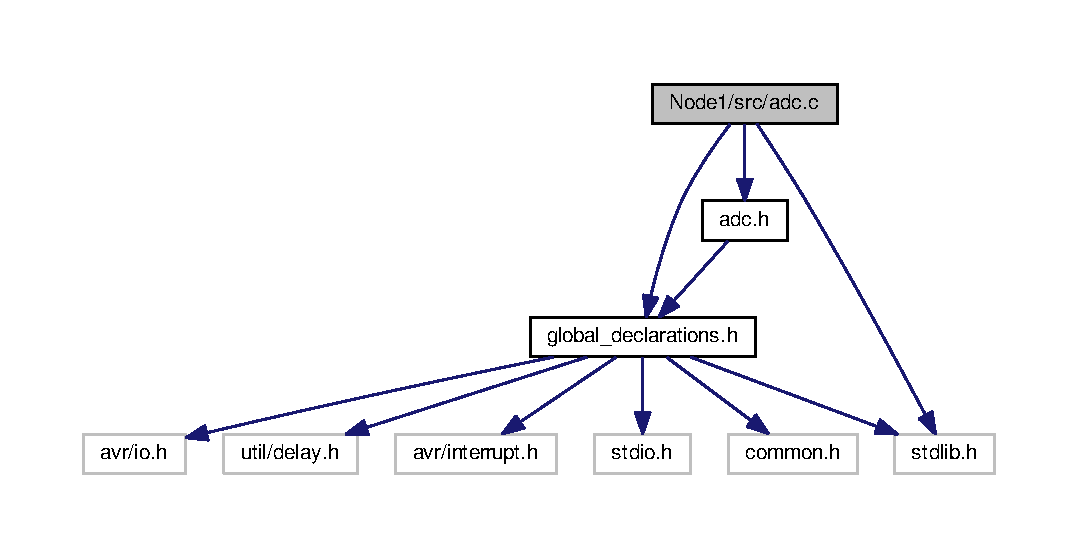
\includegraphics[width=350pt]{adc_8c__incl}
\end{center}
\end{figure}
\subsection*{Functions}
\begin{DoxyCompactItemize}
\item 
void \hyperlink{adc_8c_a2b815e6730e8723a6d1d06d9ef8f31c0}{adc\+\_\+init} (void)
\item 
uint8\+\_\+t \hyperlink{adc_8c_a725a5b40af6cdfd530ede39488b8675c}{adc\+\_\+read\+\_\+channel} (uint8\+\_\+t ch)
\end{DoxyCompactItemize}
\subsection*{Variables}
\begin{DoxyCompactItemize}
\item 
volatile uint8\+\_\+t $\ast$ {\bfseries adc\+\_\+adr} = (uint8\+\_\+t$\ast$)\hyperlink{adc_8h_a26ab0faabfa984748917473e0caffa4d}{A\+D\+C\+\_\+\+A\+DR}\hypertarget{adc_8c_adad548a663a464378b15111413d279a3}{}\label{adc_8c_adad548a663a464378b15111413d279a3}

\end{DoxyCompactItemize}


\subsection{Function Documentation}
\index{adc.\+c@{adc.\+c}!adc\+\_\+init@{adc\+\_\+init}}
\index{adc\+\_\+init@{adc\+\_\+init}!adc.\+c@{adc.\+c}}
\subsubsection[{\texorpdfstring{adc\+\_\+init(void)}{adc_init(void)}}]{\setlength{\rightskip}{0pt plus 5cm}void adc\+\_\+init (
\begin{DoxyParamCaption}
\item[{void}]{}
\end{DoxyParamCaption}
)}\hypertarget{adc_8c_a2b815e6730e8723a6d1d06d9ef8f31c0}{}\label{adc_8c_a2b815e6730e8723a6d1d06d9ef8f31c0}
Initialize mcu to interface with adc with Port D pin 2. \index{adc.\+c@{adc.\+c}!adc\+\_\+read\+\_\+channel@{adc\+\_\+read\+\_\+channel}}
\index{adc\+\_\+read\+\_\+channel@{adc\+\_\+read\+\_\+channel}!adc.\+c@{adc.\+c}}
\subsubsection[{\texorpdfstring{adc\+\_\+read\+\_\+channel(uint8\+\_\+t ch)}{adc_read_channel(uint8_t ch)}}]{\setlength{\rightskip}{0pt plus 5cm}uint8\+\_\+t adc\+\_\+read\+\_\+channel (
\begin{DoxyParamCaption}
\item[{uint8\+\_\+t}]{}
\end{DoxyParamCaption}
)}\hypertarget{adc_8c_a725a5b40af6cdfd530ede39488b8675c}{}\label{adc_8c_a725a5b40af6cdfd530ede39488b8675c}
Read analog signal at specified channel. No input validation is performed, 
\begin{DoxyParams}[1]{Parameters}
\mbox{\tt in}  & {\em ch} & uint8 in range 0 through 3. Channel that adc will perform conversion on. \\
\hline
\end{DoxyParams}

\begin{DoxyRetVals}{Return values}
{\em result} & of AD conversion \\
\hline
\end{DoxyRetVals}

\hypertarget{adc_8h}{}\section{Node1/src/adc.h File Reference}
\label{adc_8h}\index{Node1/src/adc.\+h@{Node1/src/adc.\+h}}
{\ttfamily \#include \char`\"{}global\+\_\+declarations.\+h\char`\"{}}\\*
Include dependency graph for adc.\+h\+:
\nopagebreak
\begin{figure}[H]
\begin{center}
\leavevmode
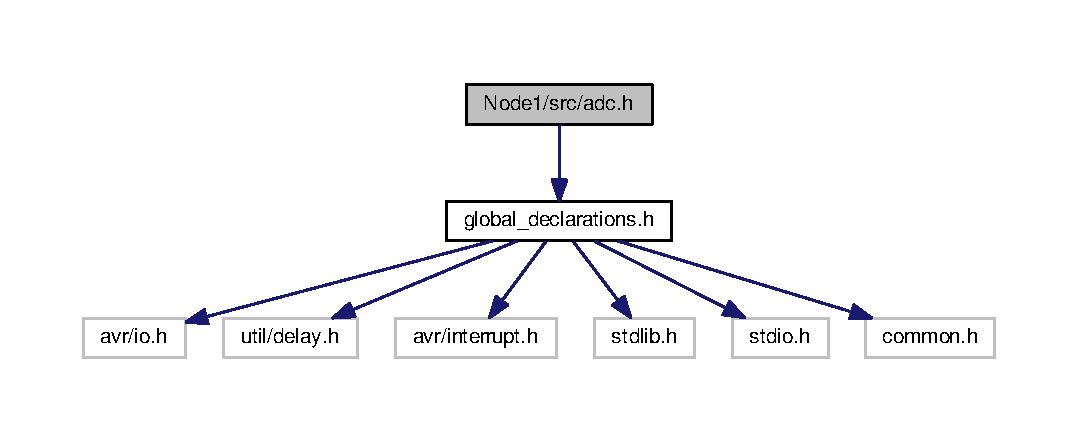
\includegraphics[width=350pt]{adc_8h__incl}
\end{center}
\end{figure}
This graph shows which files directly or indirectly include this file\+:
\nopagebreak
\begin{figure}[H]
\begin{center}
\leavevmode
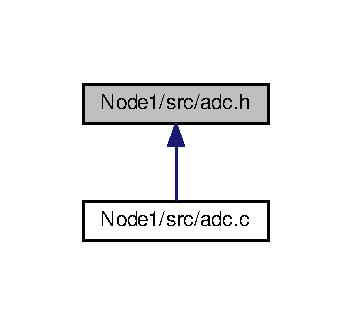
\includegraphics[width=169pt]{adc_8h__dep__incl}
\end{center}
\end{figure}
\subsection*{Macros}
\begin{DoxyCompactItemize}
\item 
\#define \hyperlink{adc_8h_a26ab0faabfa984748917473e0caffa4d}{A\+D\+C\+\_\+\+A\+DR}~0x1100
\end{DoxyCompactItemize}
\subsection*{Functions}
\begin{DoxyCompactItemize}
\item 
void \hyperlink{adc_8h_a2b815e6730e8723a6d1d06d9ef8f31c0}{adc\+\_\+init} (void)
\item 
uint8\+\_\+t \hyperlink{adc_8h_ac223c2e32d5703cfb23a4f8b3e3e3b3e}{adc\+\_\+read\+\_\+channel} (uint8\+\_\+t)
\end{DoxyCompactItemize}


\subsection{Macro Definition Documentation}
\index{adc.\+h@{adc.\+h}!A\+D\+C\+\_\+\+A\+DR@{A\+D\+C\+\_\+\+A\+DR}}
\index{A\+D\+C\+\_\+\+A\+DR@{A\+D\+C\+\_\+\+A\+DR}!adc.\+h@{adc.\+h}}
\subsubsection[{\texorpdfstring{A\+D\+C\+\_\+\+A\+DR}{ADC_ADR}}]{\setlength{\rightskip}{0pt plus 5cm}\#define A\+D\+C\+\_\+\+A\+DR~0x1100}\hypertarget{adc_8h_a26ab0faabfa984748917473e0caffa4d}{}\label{adc_8h_a26ab0faabfa984748917473e0caffa4d}
Defines an interface for external AD converter using memory mapped IO. NB\+: AD conversion is only initated when requested, and this is a blocking process. 

\subsection{Function Documentation}
\index{adc.\+h@{adc.\+h}!adc\+\_\+init@{adc\+\_\+init}}
\index{adc\+\_\+init@{adc\+\_\+init}!adc.\+h@{adc.\+h}}
\subsubsection[{\texorpdfstring{adc\+\_\+init(void)}{adc_init(void)}}]{\setlength{\rightskip}{0pt plus 5cm}void adc\+\_\+init (
\begin{DoxyParamCaption}
\item[{void}]{}
\end{DoxyParamCaption}
)}\hypertarget{adc_8h_a2b815e6730e8723a6d1d06d9ef8f31c0}{}\label{adc_8h_a2b815e6730e8723a6d1d06d9ef8f31c0}
Initialize mcu to interface with adc with Port D pin 2. \index{adc.\+h@{adc.\+h}!adc\+\_\+read\+\_\+channel@{adc\+\_\+read\+\_\+channel}}
\index{adc\+\_\+read\+\_\+channel@{adc\+\_\+read\+\_\+channel}!adc.\+h@{adc.\+h}}
\subsubsection[{\texorpdfstring{adc\+\_\+read\+\_\+channel(uint8\+\_\+t)}{adc_read_channel(uint8_t)}}]{\setlength{\rightskip}{0pt plus 5cm}uint8\+\_\+t adc\+\_\+read\+\_\+channel (
\begin{DoxyParamCaption}
\item[{uint8\+\_\+t}]{}
\end{DoxyParamCaption}
)}\hypertarget{adc_8h_ac223c2e32d5703cfb23a4f8b3e3e3b3e}{}\label{adc_8h_ac223c2e32d5703cfb23a4f8b3e3e3b3e}
Read analog signal at specified channel. No input validation is performed, 
\begin{DoxyParams}[1]{Parameters}
\mbox{\tt in}  & {\em ch} & uint8 in range 0 through 3. Channel that adc will perform conversion on. \\
\hline
\end{DoxyParams}

\begin{DoxyRetVals}{Return values}
{\em result} & of AD conversion \\
\hline
\end{DoxyRetVals}

\hypertarget{Node1_2src_2uart_8c}{}\section{Node1/src/uart.c File Reference}
\label{Node1_2src_2uart_8c}\index{Node1/src/uart.\+c@{Node1/src/uart.\+c}}
{\ttfamily \#include \char`\"{}global\+\_\+declarations.\+h\char`\"{}}\\*
{\ttfamily \#include $<$avr/io.\+h$>$}\\*
{\ttfamily \#include $<$avr/interrupt.\+h$>$}\\*
{\ttfamily \#include $<$stdio.\+h$>$}\\*
{\ttfamily \#include $<$stdlib.\+h$>$}\\*
{\ttfamily \#include $<$string.\+h$>$}\\*
{\ttfamily \#include \char`\"{}uart.\+h\char`\"{}}\\*
Include dependency graph for uart.\+c\+:
\nopagebreak
\begin{figure}[H]
\begin{center}
\leavevmode
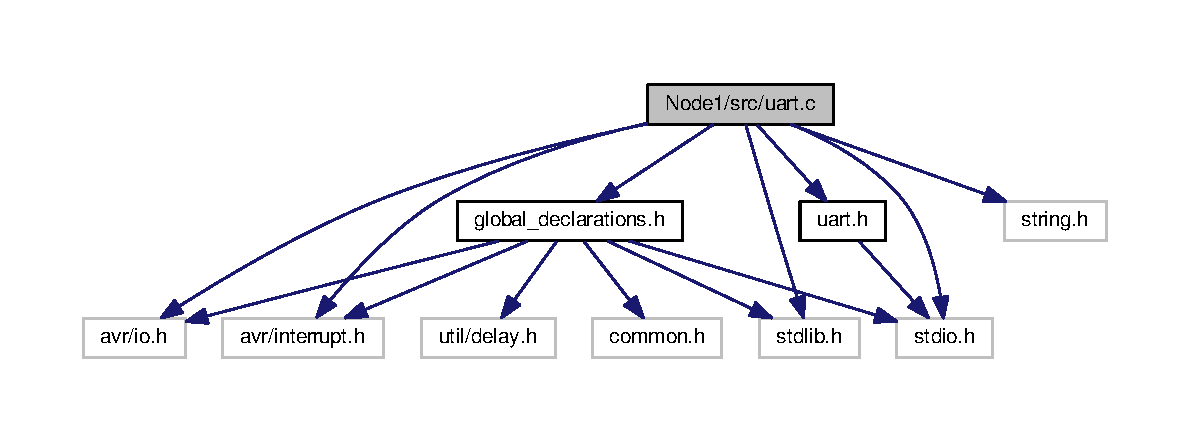
\includegraphics[width=350pt]{Node1_2src_2uart_8c__incl}
\end{center}
\end{figure}
\subsection*{Macros}
\begin{DoxyCompactItemize}
\item 
\#define {\bfseries B\+A\+UD}~9600\+U\+L 	/$\ast$! B\+A\+U\+D rate of U\+A\+R\+T$\ast$/\hypertarget{Node1_2src_2uart_8c_a62634036639f88eece6fbf226b45f84b}{}\label{Node1_2src_2uart_8c_a62634036639f88eece6fbf226b45f84b}

\item 
\#define {\bfseries B\+U\+F\+F\+E\+R\+\_\+\+M\+AX}~128 	/$\ast$! Size of Rx buffer$\ast$/\hypertarget{Node1_2src_2uart_8c_a65c660282414eff7e990f21f6b306cb8}{}\label{Node1_2src_2uart_8c_a65c660282414eff7e990f21f6b306cb8}

\end{DoxyCompactItemize}
\subsection*{Functions}
\begin{DoxyCompactItemize}
\item 
\hyperlink{Node1_2src_2uart_8c_a9622edb266a65452131cdbbccb5e5b0e}{I\+SR} (U\+S\+A\+R\+T0\+\_\+\+R\+X\+C\+\_\+vect)
\begin{DoxyCompactList}\small\item\em Interrupt vector for Rx. Place recieved data into buffer. \end{DoxyCompactList}\item 
\hyperlink{Node1_2src_2uart_8c_ae386730179b92f3cd381054196cc0751}{I\+SR} (U\+S\+A\+R\+T0\+\_\+\+T\+X\+C\+\_\+vect)
\item 
void \hyperlink{Node1_2src_2uart_8c_a01f5996cfbcef121abc486e732b208c7}{uart\+\_\+init} ()
\begin{DoxyCompactList}\small\item\em Initialize uart. \end{DoxyCompactList}\item 
int \hyperlink{Node1_2src_2uart_8c_a3997eef358f90d23280d1108a32d85e7}{uart\+\_\+send} (unsigned char msg)
\begin{DoxyCompactList}\small\item\em Busy wait transmission of msg. \end{DoxyCompactList}\item 
unsigned char \hyperlink{Node1_2src_2uart_8c_a1127aebe7441e1cc25f738127c53c4a3}{uart\+\_\+recv} ()
\begin{DoxyCompactList}\small\item\em Read data from buffer. \end{DoxyCompactList}\end{DoxyCompactItemize}
\subsection*{Variables}
\begin{DoxyCompactItemize}
\item 
F\+I\+LE \hyperlink{Node1_2src_2uart_8c_af7b899691fa46afc4d24937667462b08}{uart\+\_\+out} = F\+D\+E\+V\+\_\+\+S\+E\+T\+U\+P\+\_\+\+S\+T\+R\+E\+AM(\hyperlink{Node1_2src_2uart_8h_a3997eef358f90d23280d1108a32d85e7}{uart\+\_\+send}, N\+U\+LL, \+\_\+\+F\+D\+E\+V\+\_\+\+S\+E\+T\+U\+P\+\_\+\+W\+R\+I\+TE)
\begin{DoxyCompactList}\small\item\em Enable use of fprintf(\&uart\+\_\+out,...) for. \end{DoxyCompactList}\item 
F\+I\+LE \hyperlink{Node1_2src_2uart_8c_a40f1986412d89052918098aaf10377e5}{uart\+\_\+in} = F\+D\+E\+V\+\_\+\+S\+E\+T\+U\+P\+\_\+\+S\+T\+R\+E\+AM(N\+U\+LL, \hyperlink{Node1_2src_2uart_8h_a1127aebe7441e1cc25f738127c53c4a3}{uart\+\_\+recv}, \+\_\+\+F\+D\+E\+V\+\_\+\+S\+E\+T\+U\+P\+\_\+\+R\+E\+AD)\hypertarget{Node1_2src_2uart_8c_a40f1986412d89052918098aaf10377e5}{}\label{Node1_2src_2uart_8c_a40f1986412d89052918098aaf10377e5}

\begin{DoxyCompactList}\small\item\em Create input stream for uart. Unused. \end{DoxyCompactList}\item 
volatile char {\bfseries recv\+\_\+buffer} \mbox{[}B\+U\+F\+F\+E\+R\+\_\+\+M\+AX\mbox{]}\hypertarget{Node1_2src_2uart_8c_a2fa9595c8e9f9ba1955e5a427845ea4f}{}\label{Node1_2src_2uart_8c_a2fa9595c8e9f9ba1955e5a427845ea4f}

\item 
volatile int \hyperlink{Node1_2src_2uart_8c_aa4b36744e9b33682a6c02c5463ba28cf}{recvhead} = 0
\item 
volatile int \hyperlink{Node1_2src_2uart_8c_a3220abd95746b723680be6bc93ab26f7}{recvtail} = 0
\end{DoxyCompactItemize}


\subsection{Function Documentation}
\index{Node1/src/uart.\+c@{Node1/src/uart.\+c}!I\+SR@{I\+SR}}
\index{I\+SR@{I\+SR}!Node1/src/uart.\+c@{Node1/src/uart.\+c}}
\subsubsection[{\texorpdfstring{I\+S\+R(\+U\+S\+A\+R\+T0\+\_\+\+R\+X\+C\+\_\+vect)}{ISR(USART0_RXC_vect)}}]{\setlength{\rightskip}{0pt plus 5cm}I\+SR (
\begin{DoxyParamCaption}
\item[{U\+S\+A\+R\+T0\+\_\+\+R\+X\+C\+\_\+vect}]{}
\end{DoxyParamCaption}
)}\hypertarget{Node1_2src_2uart_8c_a9622edb266a65452131cdbbccb5e5b0e}{}\label{Node1_2src_2uart_8c_a9622edb266a65452131cdbbccb5e5b0e}


Interrupt vector for Rx. Place recieved data into buffer. 

Tail of buffer. Where next read will occour. \index{Node1/src/uart.\+c@{Node1/src/uart.\+c}!I\+SR@{I\+SR}}
\index{I\+SR@{I\+SR}!Node1/src/uart.\+c@{Node1/src/uart.\+c}}
\subsubsection[{\texorpdfstring{I\+S\+R(\+U\+S\+A\+R\+T0\+\_\+\+T\+X\+C\+\_\+vect)}{ISR(USART0_TXC_vect)}}]{\setlength{\rightskip}{0pt plus 5cm}I\+SR (
\begin{DoxyParamCaption}
\item[{U\+S\+A\+R\+T0\+\_\+\+T\+X\+C\+\_\+vect}]{}
\end{DoxyParamCaption}
)}\hypertarget{Node1_2src_2uart_8c_ae386730179b92f3cd381054196cc0751}{}\label{Node1_2src_2uart_8c_ae386730179b92f3cd381054196cc0751}
\begin{DoxyRefDesc}{Todo}
\item[\hyperlink{todo__todo000001}{Todo}]remove interrupt from Tx \end{DoxyRefDesc}
\index{Node1/src/uart.\+c@{Node1/src/uart.\+c}!uart\+\_\+init@{uart\+\_\+init}}
\index{uart\+\_\+init@{uart\+\_\+init}!Node1/src/uart.\+c@{Node1/src/uart.\+c}}
\subsubsection[{\texorpdfstring{uart\+\_\+init()}{uart_init()}}]{\setlength{\rightskip}{0pt plus 5cm}void uart\+\_\+init (
\begin{DoxyParamCaption}
{}
\end{DoxyParamCaption}
)}\hypertarget{Node1_2src_2uart_8c_a01f5996cfbcef121abc486e732b208c7}{}\label{Node1_2src_2uart_8c_a01f5996cfbcef121abc486e732b208c7}


Initialize uart. 

Initialize U\+A\+RT. \index{Node1/src/uart.\+c@{Node1/src/uart.\+c}!uart\+\_\+recv@{uart\+\_\+recv}}
\index{uart\+\_\+recv@{uart\+\_\+recv}!Node1/src/uart.\+c@{Node1/src/uart.\+c}}
\subsubsection[{\texorpdfstring{uart\+\_\+recv()}{uart_recv()}}]{\setlength{\rightskip}{0pt plus 5cm}unsigned char uart\+\_\+recv (
\begin{DoxyParamCaption}
{}
\end{DoxyParamCaption}
)}\hypertarget{Node1_2src_2uart_8c_a1127aebe7441e1cc25f738127c53c4a3}{}\label{Node1_2src_2uart_8c_a1127aebe7441e1cc25f738127c53c4a3}


Read data from buffer. 

Read one byte from the Rx buffer. Return zero if buffer is empty. 
\begin{DoxyRetVals}{Return values}
{\em } & \\
\hline
\end{DoxyRetVals}
\index{Node1/src/uart.\+c@{Node1/src/uart.\+c}!uart\+\_\+send@{uart\+\_\+send}}
\index{uart\+\_\+send@{uart\+\_\+send}!Node1/src/uart.\+c@{Node1/src/uart.\+c}}
\subsubsection[{\texorpdfstring{uart\+\_\+send(unsigned char msg)}{uart_send(unsigned char msg)}}]{\setlength{\rightskip}{0pt plus 5cm}int uart\+\_\+send (
\begin{DoxyParamCaption}
\item[{unsigned char}]{msg}
\end{DoxyParamCaption}
)}\hypertarget{Node1_2src_2uart_8c_a3997eef358f90d23280d1108a32d85e7}{}\label{Node1_2src_2uart_8c_a3997eef358f90d23280d1108a32d85e7}


Busy wait transmission of msg. 

Send data 
\begin{DoxyParams}[1]{Parameters}
\mbox{\tt in}  & {\em msg} & one byte of data to send \\
\hline
\end{DoxyParams}

\begin{DoxyRetVals}{Return values}
{\em 0} & always. \\
\hline
\end{DoxyRetVals}


\subsection{Variable Documentation}
\index{Node1/src/uart.\+c@{Node1/src/uart.\+c}!recvhead@{recvhead}}
\index{recvhead@{recvhead}!Node1/src/uart.\+c@{Node1/src/uart.\+c}}
\subsubsection[{\texorpdfstring{recvhead}{recvhead}}]{\setlength{\rightskip}{0pt plus 5cm}volatile int recvhead = 0}\hypertarget{Node1_2src_2uart_8c_aa4b36744e9b33682a6c02c5463ba28cf}{}\label{Node1_2src_2uart_8c_aa4b36744e9b33682a6c02c5463ba28cf}
Buffer for storing recieved data \index{Node1/src/uart.\+c@{Node1/src/uart.\+c}!recvtail@{recvtail}}
\index{recvtail@{recvtail}!Node1/src/uart.\+c@{Node1/src/uart.\+c}}
\subsubsection[{\texorpdfstring{recvtail}{recvtail}}]{\setlength{\rightskip}{0pt plus 5cm}volatile int recvtail = 0}\hypertarget{Node1_2src_2uart_8c_a3220abd95746b723680be6bc93ab26f7}{}\label{Node1_2src_2uart_8c_a3220abd95746b723680be6bc93ab26f7}
Head of buffer. Where next recieved byte will be placed. \index{Node1/src/uart.\+c@{Node1/src/uart.\+c}!uart\+\_\+out@{uart\+\_\+out}}
\index{uart\+\_\+out@{uart\+\_\+out}!Node1/src/uart.\+c@{Node1/src/uart.\+c}}
\subsubsection[{\texorpdfstring{uart\+\_\+out}{uart_out}}]{\setlength{\rightskip}{0pt plus 5cm}F\+I\+LE uart\+\_\+out = F\+D\+E\+V\+\_\+\+S\+E\+T\+U\+P\+\_\+\+S\+T\+R\+E\+AM({\bf uart\+\_\+send}, N\+U\+LL, \+\_\+\+F\+D\+E\+V\+\_\+\+S\+E\+T\+U\+P\+\_\+\+W\+R\+I\+TE)}\hypertarget{Node1_2src_2uart_8c_af7b899691fa46afc4d24937667462b08}{}\label{Node1_2src_2uart_8c_af7b899691fa46afc4d24937667462b08}


Enable use of fprintf(\&uart\+\_\+out,...) for. 

U\+A\+RT implementation for atmega162 Hardcoded to use 9600 buad 8n1 = 8 data-\/bits, no parity, 1 stop bit Uses interrupts for recieving and busy wait for sending. Recieved messages go into an internal buffer untill mcu request them.\begin{DoxyRefDesc}{Todo}
\item[\hyperlink{todo__todo000002}{Todo}]\{change to use uint8\+\_\+t where it makes sense\} 

\{implement \char`\"{}buffer full\char`\"{} function\} \end{DoxyRefDesc}

\hypertarget{Node1_2src_2uart_8h}{}\section{Node1/src/uart.h File Reference}
\label{Node1_2src_2uart_8h}\index{Node1/src/uart.\+h@{Node1/src/uart.\+h}}
{\ttfamily \#include $<$stdio.\+h$>$}\\*
Include dependency graph for uart.\+h\+:
\nopagebreak
\begin{figure}[H]
\begin{center}
\leavevmode
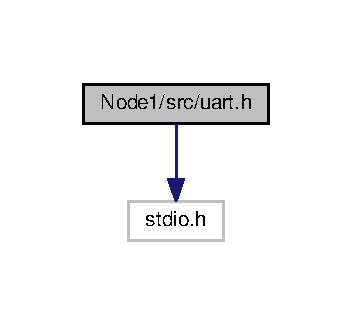
\includegraphics[width=169pt]{Node1_2src_2uart_8h__incl}
\end{center}
\end{figure}
This graph shows which files directly or indirectly include this file\+:
\nopagebreak
\begin{figure}[H]
\begin{center}
\leavevmode
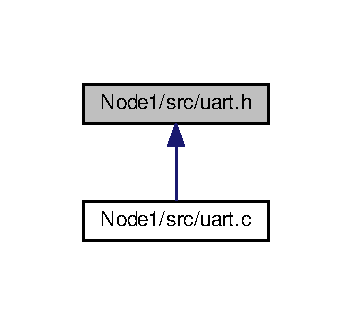
\includegraphics[width=169pt]{Node1_2src_2uart_8h__dep__incl}
\end{center}
\end{figure}
\subsection*{Functions}
\begin{DoxyCompactItemize}
\item 
void \hyperlink{Node1_2src_2uart_8h_a01f5996cfbcef121abc486e732b208c7}{uart\+\_\+init} ()
\begin{DoxyCompactList}\small\item\em Initialize uart. \end{DoxyCompactList}\item 
int \hyperlink{Node1_2src_2uart_8h_a3997eef358f90d23280d1108a32d85e7}{uart\+\_\+send} (unsigned char msg)
\begin{DoxyCompactList}\small\item\em Busy wait transmission of msg. \end{DoxyCompactList}\item 
unsigned char \hyperlink{Node1_2src_2uart_8h_a1127aebe7441e1cc25f738127c53c4a3}{uart\+\_\+recv} ()
\begin{DoxyCompactList}\small\item\em Read data from buffer. \end{DoxyCompactList}\end{DoxyCompactItemize}
\subsection*{Variables}
\begin{DoxyCompactItemize}
\item 
F\+I\+LE \hyperlink{Node1_2src_2uart_8h_af7b899691fa46afc4d24937667462b08}{uart\+\_\+out}
\begin{DoxyCompactList}\small\item\em Enable use of fprintf(\&uart\+\_\+out,...) for. \end{DoxyCompactList}\item 
F\+I\+LE \hyperlink{Node1_2src_2uart_8h_a40f1986412d89052918098aaf10377e5}{uart\+\_\+in}\hypertarget{Node1_2src_2uart_8h_a40f1986412d89052918098aaf10377e5}{}\label{Node1_2src_2uart_8h_a40f1986412d89052918098aaf10377e5}

\begin{DoxyCompactList}\small\item\em Create input stream for uart. Unused. \end{DoxyCompactList}\end{DoxyCompactItemize}


\subsection{Function Documentation}
\index{Node1/src/uart.\+h@{Node1/src/uart.\+h}!uart\+\_\+init@{uart\+\_\+init}}
\index{uart\+\_\+init@{uart\+\_\+init}!Node1/src/uart.\+h@{Node1/src/uart.\+h}}
\subsubsection[{\texorpdfstring{uart\+\_\+init()}{uart_init()}}]{\setlength{\rightskip}{0pt plus 5cm}void uart\+\_\+init (
\begin{DoxyParamCaption}
{}
\end{DoxyParamCaption}
)}\hypertarget{Node1_2src_2uart_8h_a01f5996cfbcef121abc486e732b208c7}{}\label{Node1_2src_2uart_8h_a01f5996cfbcef121abc486e732b208c7}


Initialize uart. 

Initialize U\+A\+RT. \index{Node1/src/uart.\+h@{Node1/src/uart.\+h}!uart\+\_\+recv@{uart\+\_\+recv}}
\index{uart\+\_\+recv@{uart\+\_\+recv}!Node1/src/uart.\+h@{Node1/src/uart.\+h}}
\subsubsection[{\texorpdfstring{uart\+\_\+recv()}{uart_recv()}}]{\setlength{\rightskip}{0pt plus 5cm}unsigned char uart\+\_\+recv (
\begin{DoxyParamCaption}
{}
\end{DoxyParamCaption}
)}\hypertarget{Node1_2src_2uart_8h_a1127aebe7441e1cc25f738127c53c4a3}{}\label{Node1_2src_2uart_8h_a1127aebe7441e1cc25f738127c53c4a3}


Read data from buffer. 

Read one byte from the Rx buffer. Return zero if buffer is empty. 
\begin{DoxyRetVals}{Return values}
{\em } & \\
\hline
\end{DoxyRetVals}
\index{Node1/src/uart.\+h@{Node1/src/uart.\+h}!uart\+\_\+send@{uart\+\_\+send}}
\index{uart\+\_\+send@{uart\+\_\+send}!Node1/src/uart.\+h@{Node1/src/uart.\+h}}
\subsubsection[{\texorpdfstring{uart\+\_\+send(unsigned char msg)}{uart_send(unsigned char msg)}}]{\setlength{\rightskip}{0pt plus 5cm}int uart\+\_\+send (
\begin{DoxyParamCaption}
\item[{unsigned char}]{msg}
\end{DoxyParamCaption}
)}\hypertarget{Node1_2src_2uart_8h_a3997eef358f90d23280d1108a32d85e7}{}\label{Node1_2src_2uart_8h_a3997eef358f90d23280d1108a32d85e7}


Busy wait transmission of msg. 

Send data 
\begin{DoxyParams}[1]{Parameters}
\mbox{\tt in}  & {\em msg} & one byte of data to send \\
\hline
\end{DoxyParams}

\begin{DoxyRetVals}{Return values}
{\em 0} & always. \\
\hline
\end{DoxyRetVals}


\subsection{Variable Documentation}
\index{Node1/src/uart.\+h@{Node1/src/uart.\+h}!uart\+\_\+out@{uart\+\_\+out}}
\index{uart\+\_\+out@{uart\+\_\+out}!Node1/src/uart.\+h@{Node1/src/uart.\+h}}
\subsubsection[{\texorpdfstring{uart\+\_\+out}{uart_out}}]{\setlength{\rightskip}{0pt plus 5cm}F\+I\+LE uart\+\_\+out}\hypertarget{Node1_2src_2uart_8h_af7b899691fa46afc4d24937667462b08}{}\label{Node1_2src_2uart_8h_af7b899691fa46afc4d24937667462b08}


Enable use of fprintf(\&uart\+\_\+out,...) for. 

U\+A\+RT implementation for atmega162 Hardcoded to use 9600 buad 8n1 = 8 data-\/bits, no parity, 1 stop bit Uses interrupts for recieving and busy wait for sending. Recieved messages go into an internal buffer untill mcu request them.\begin{DoxyRefDesc}{Todo}
\item[\hyperlink{todo__todo000002}{Todo}]\{change to use uint8\+\_\+t where it makes sense\} 

\{implement \char`\"{}buffer full\char`\"{} function\} \end{DoxyRefDesc}

%--- End generated contents ---

% Index
\backmatter
\newpage
\phantomsection
\clearemptydoublepage
\addcontentsline{toc}{chapter}{Index}
\printindex

\end{document}
